\label{sec:results}

\subsection{Algorithm on real data}

In this section we show the first results obtained from the first part of the commissioning campaign of the instrument, installed at the QUIJOTE telescope in Tenerife. We can see in fig. \ref{fig:circle} the circular fit performed on real data as described in fig. \ref{fig:IQ_modulation}: the two external are the modulation points and the central distribution represents the variation of the signal during the observations.


\begin{figure}[htf]
	\centering
	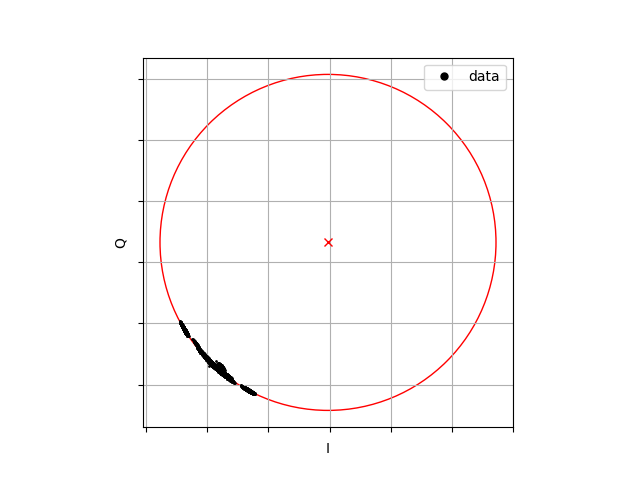
\includegraphics[width=.5\textwidth]{4.results/circular_fit.png}
	\caption{Observation in $(I,Q)$ plan: in black dots the data and in red shape the circular fit. We can see the two modulation (external) points and the central distribution due to the signal changing during the observation [scan 283, pixel KA001]}
	\label{fig:circle}
\end{figure}

\noindent Operatively, the circular fit showed in fig. \ref{fig:circle} is used in two different ways and represents a crucial tool during the observations, as well as for the data analysis. Firstly, during the observation, it gives an important visual feedback to understand if the tuning (as seen in sec. \ref{sec:tuning} ) is correctly working. Secondly, it is one of the first step in the conversion algorithm for the physical data analysis, as already described in sec. \ref{sebsec:alg}.

The first result, that we can compare with the simulation, is reported in fig. \ref{fig:calfact}: it is the calibration factor estimated as a function of TOI during a sky observation. Every point corresponds to a data block (sampled at 5 Hz).

\begin{figure}[htf]
	\centering
	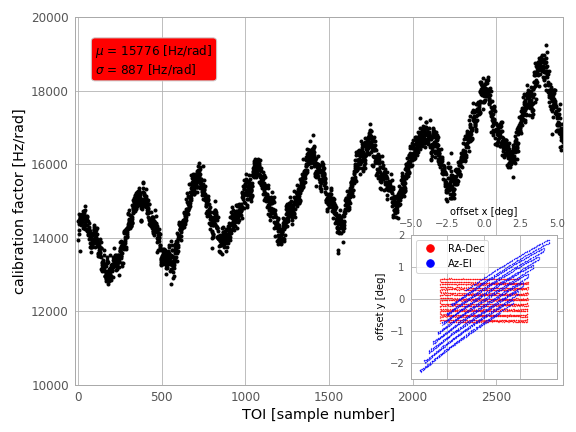
\includegraphics[width=.7\textwidth]{4.results/calfact.png}
	\caption{Calibration factor as a function of Time Ordered Information, TOI, during an observation. The gaussian fit reported in the red top-left box is evaluated from the data that have beed before median filtered. We can notice the derive of the calibration factor due to the Right-Ascension Declination (RA-Dec) observation: the telescope increases the elevation following the source. In the bottom-right the offset maps of the sky-coordinates in RA-Dec and Azimuth-Elevation.}
	\label{fig:calfact}
\end{figure}


Here we assume the background fluctuation, as seen in fig. \ref{fig:cal_bck}, as unique source of incertitude for the calibration factor estimation: we consider the noise contamination negligible, let's first demonstrate this assumption. We take the median of the $ASD$, $\tilde{ASD}$, as its equivalent white noise level: it is (taking margins) $\sim$1 $Hz/\sqrt{Hz}$.

\noindent  We can, then, use the definition of the standard deviation of the TOI noise signal:

\begin{equation}
\sigma \doteq \int_{0}^{\Delta f} [ASD(f)]^2\cdot df \text{ ,}
\label{eq:sigma}
\end{equation}

\noindent where $ASD(f)$ is the $ASD$ as a function of frequency $f\in[0,\Delta f]$, $\Delta f$ is the bandwidth equal to half of the sampling frequency (for the Nyquist theorem) and $df\doteq\Delta f/N$, with $N$ is the number of the points.

\noindent Approximating $ASD$ in eq. \ref{eq:sigma} as a pure white noise, $\tilde{ASD}$, we obtain:

\begin{equation}
\sigma\simeq \sqrt{ \tilde{ASD}^2 \cdot \Delta f } \text{ ,}
\end{equation}

\noindent Finally, in tab. \ref{tab:sigma_sig}, we can see the typical fluctuations of the signal as a function of sampling rate: compared to the background variation (equivalent of $\sim 1$ kHz) simulation in fig. \ref{fig:calfact} it represents, Q.E.D., a very small components.

\begin{table}[htf]
	\footnotesize
	\centering
	\caption{From eq. \ref{eq:sigma} typical rounded-up 1-$\sigma$ noise signal.}
	\begin{tabular}{ccc}
		\toprule
		\textbf{mode} & \textbf{bandwidth [Hz]} & \textbf{$\sigma$ [Hz]} \\
		\toprule
		single point & 1908 & $\sim$50 \\ 
		\midrule 
		block data & 2 & $\sim$2 \\ 
		\bottomrule
	\end{tabular}
	\label{tab:sigma_sig}
\end{table}

Starting from this paradigm we can, thus, compare the results of the simulation with on sky observations. In the first scenario there is a $\lesssim 3\%$ variation of the calibration factor each kelvin background fluctuation, as shown in fig. \ref{fig:cal_bck}. What we notice on sky (fig. \ref{fig:calfact}) is a fluctuation $\sigma/\mu\sim6\%$, where $\sigma$ is the standard deviation and $\mu$ the mean value of the calibration factor. We can conclude that during a typical $\sim$4$\textdegree$ scan we have temperature fluctuation of the sky $\lesssim 2$ K.


\subsection{Algorithm validation}
The purpose of this study is to qualify the new technique developed for KISS: modulation and auto-tuning.

\color{red}
To insert validation of calibration.
\color{black}

Secondly, what we need to state that the acquisition/data-reduction system is qualified for the instrument is to observe if the auto-tuning (sec. \ref{sec:tuning}) works. For this purpose, we take three consecutive maps at different elevations: we plot the $(I,Q)$ data of the first subscan for each map observing the behaviour of the acquisition referring the circular fit to the first tuning (corresponding to the first map). The result is shown in fig. \ref{fig:autotuning}.

\begin{figure}[htf]
	\centering
	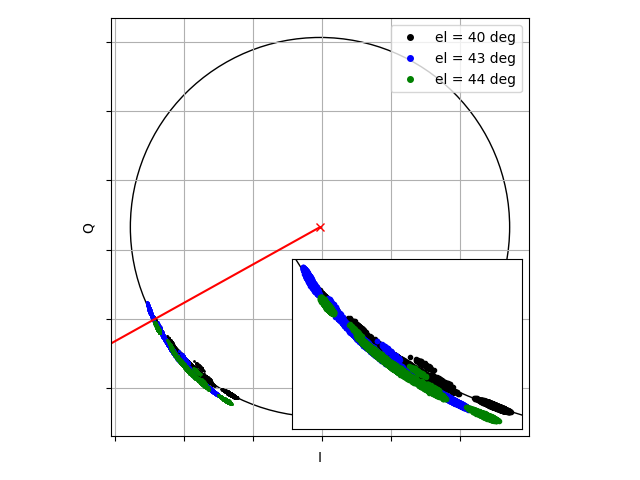
\includegraphics[width=.5\textwidth]{4.results/autotuning.png}
	\caption{$(I,Q)$ signal of the first subscan for three consecutive maps, i.e., different elevations. The red straight line is the intercept between the origin and the circle centre.}
	\label{fig:autotuning}
\end{figure}

\noindent We can see how the data are disposed on the same region close to the ones of the first circle, they are around the intercept between the centre of the circle the origin: it means that they are around the minimum of the resonance, i.e., to the frequency of resonance. The data are not perfectly centred because of the intrinsic incertitude on the binning of the injected tone. The radial shift is due to the background change: different elevations correspond to a different air mass, $\sim 1/\cos(el)$. The tuning technique performed between each map recover the resonance  tone, adapting it to the background change.